\documentclass[11pt,letterpaper]{article}
\usepackage{graphicx}
\usepackage{geometry}
\usepackage{amsmath}
\usepackage{amssymb}
\usepackage{hyperref}
\usepackage{url}
\usepackage{natbib}
\usepackage{booktabs}
\usepackage{xcolor}
\usepackage{listings}
\usepackage{microtype}
\usepackage{parskip}

\geometry{margin=1in}
\hypersetup{colorlinks=true, linkcolor=black, citecolor=blue, urlcolor=blue}

\title{\textbf{Hodge Decomposition for Citation Cartel Detection}}

\author{Anonymous Author(s)}

\date{}

\begin{document}

\maketitle

\begin{abstract}
Citation cartels---organized groups of journals coordinating excessive mutual citations---distort the scientific record and misallocate research funding. Existing detection methods rely on threshold-based heuristics or null models that paradoxically suppress cartel signals in large journals. We propose Citation Vortex Score (CVS), a parameter-free detector grounded in Hodge decomposition from algebraic topology. CVS decomposes journal-level citation flow into gradient (acyclic prestige-driven citations) and residual (circulation) components, scoring subgroups by the fraction of non-gradient flow. On synthetic data with ground-truth cartels at $15\times$ citation boost, CVS achieves AUC-ROC$=1.000$ versus $0.892$ for reciprocity ratio and $0.0$ for degree-corrected baselines. The method demonstrates high temporal stability (Spearman $\rho=0.939$) and robustness across community detection algorithms. CVS requires no null model tuning, no training data, and no threshold selection---only sparse linear algebra and community detection from standard libraries. Real-world validation on Clarivate-suppressed journals remains future work, but synthetic results and theoretical grounding in Hodge theory suggest CVS offers a principled alternative to statistical null models for network anomaly detection.
\end{abstract}

\section{Introduction}

Academic citation networks form the foundation of scientific reputation and resource allocation. The Journal Impact Factor (JIF)---the mean number of citations a journal receives annually---directly influences research funding, hiring decisions, and institutional rankings. This high-stakes system creates perverse incentives: organized groups of journals can artificially inflate their impact factors through citation cartels---coordinated networks of mutual citation exchanges at artificially high rates. Clarivate, the authority publishing Journal Citation Reports, has suspended approximately 20 journals annually in recent years for excessive self-citation and citation stacking, suggesting the problem is widespread and accelerating \citep{Kojaku2021}.

Citation cartels damage science in multiple ways. They crowd out citations to foundational work, misrepresent research importance, and redirect both reader attention and funding toward a narrow set of journals. A typical cartel comprises 2--10 journals, with 30--50\% or more of incoming citations from within-group sources---far above normal disciplinary norms \citep{Kojaku2021}.

The scientific challenge is detection. Existing methods fall into two categories, each with critical limitations. \textbf{Threshold-based approaches} identify journal pairs with excessive mutual citations, but ignore network context and miss multi-step cycles (A$\to$B$\to$C$\to$A) that characterize sophisticated cartels. \textbf{Statistical null-model approaches} like the degree-corrected stochastic block model (dcSBM, used in CIDRE) explicitly expect high mutual citations among large, active journals, potentially normalizing away the cartel signal by design \citep{Kojaku2021}. Neither method is parameter-free or fully transparent.

We propose a fundamentally different approach: \textbf{Citation Vortex Score (CVS)}, grounded in Hodge decomposition from algebraic topology. The mathematical insight is that flow on any directed graph decomposes uniquely into three orthogonal components: (1)~\textbf{gradient flow}---acyclic hierarchical patterns reflecting legitimate prestige hierarchies; (2)~\textbf{curl flow}---locally rotational patterns reflecting citation cartels; and (3)~\textbf{harmonic flow}---globally cyclic but locally consistent patterns. By measuring the ratio of non-gradient (residual) energy to total energy within journal communities, we obtain a parameter-free, interpretable cartel score requiring no null model tuning and no training data.

\begin{figure*}[!t]
  \centering
  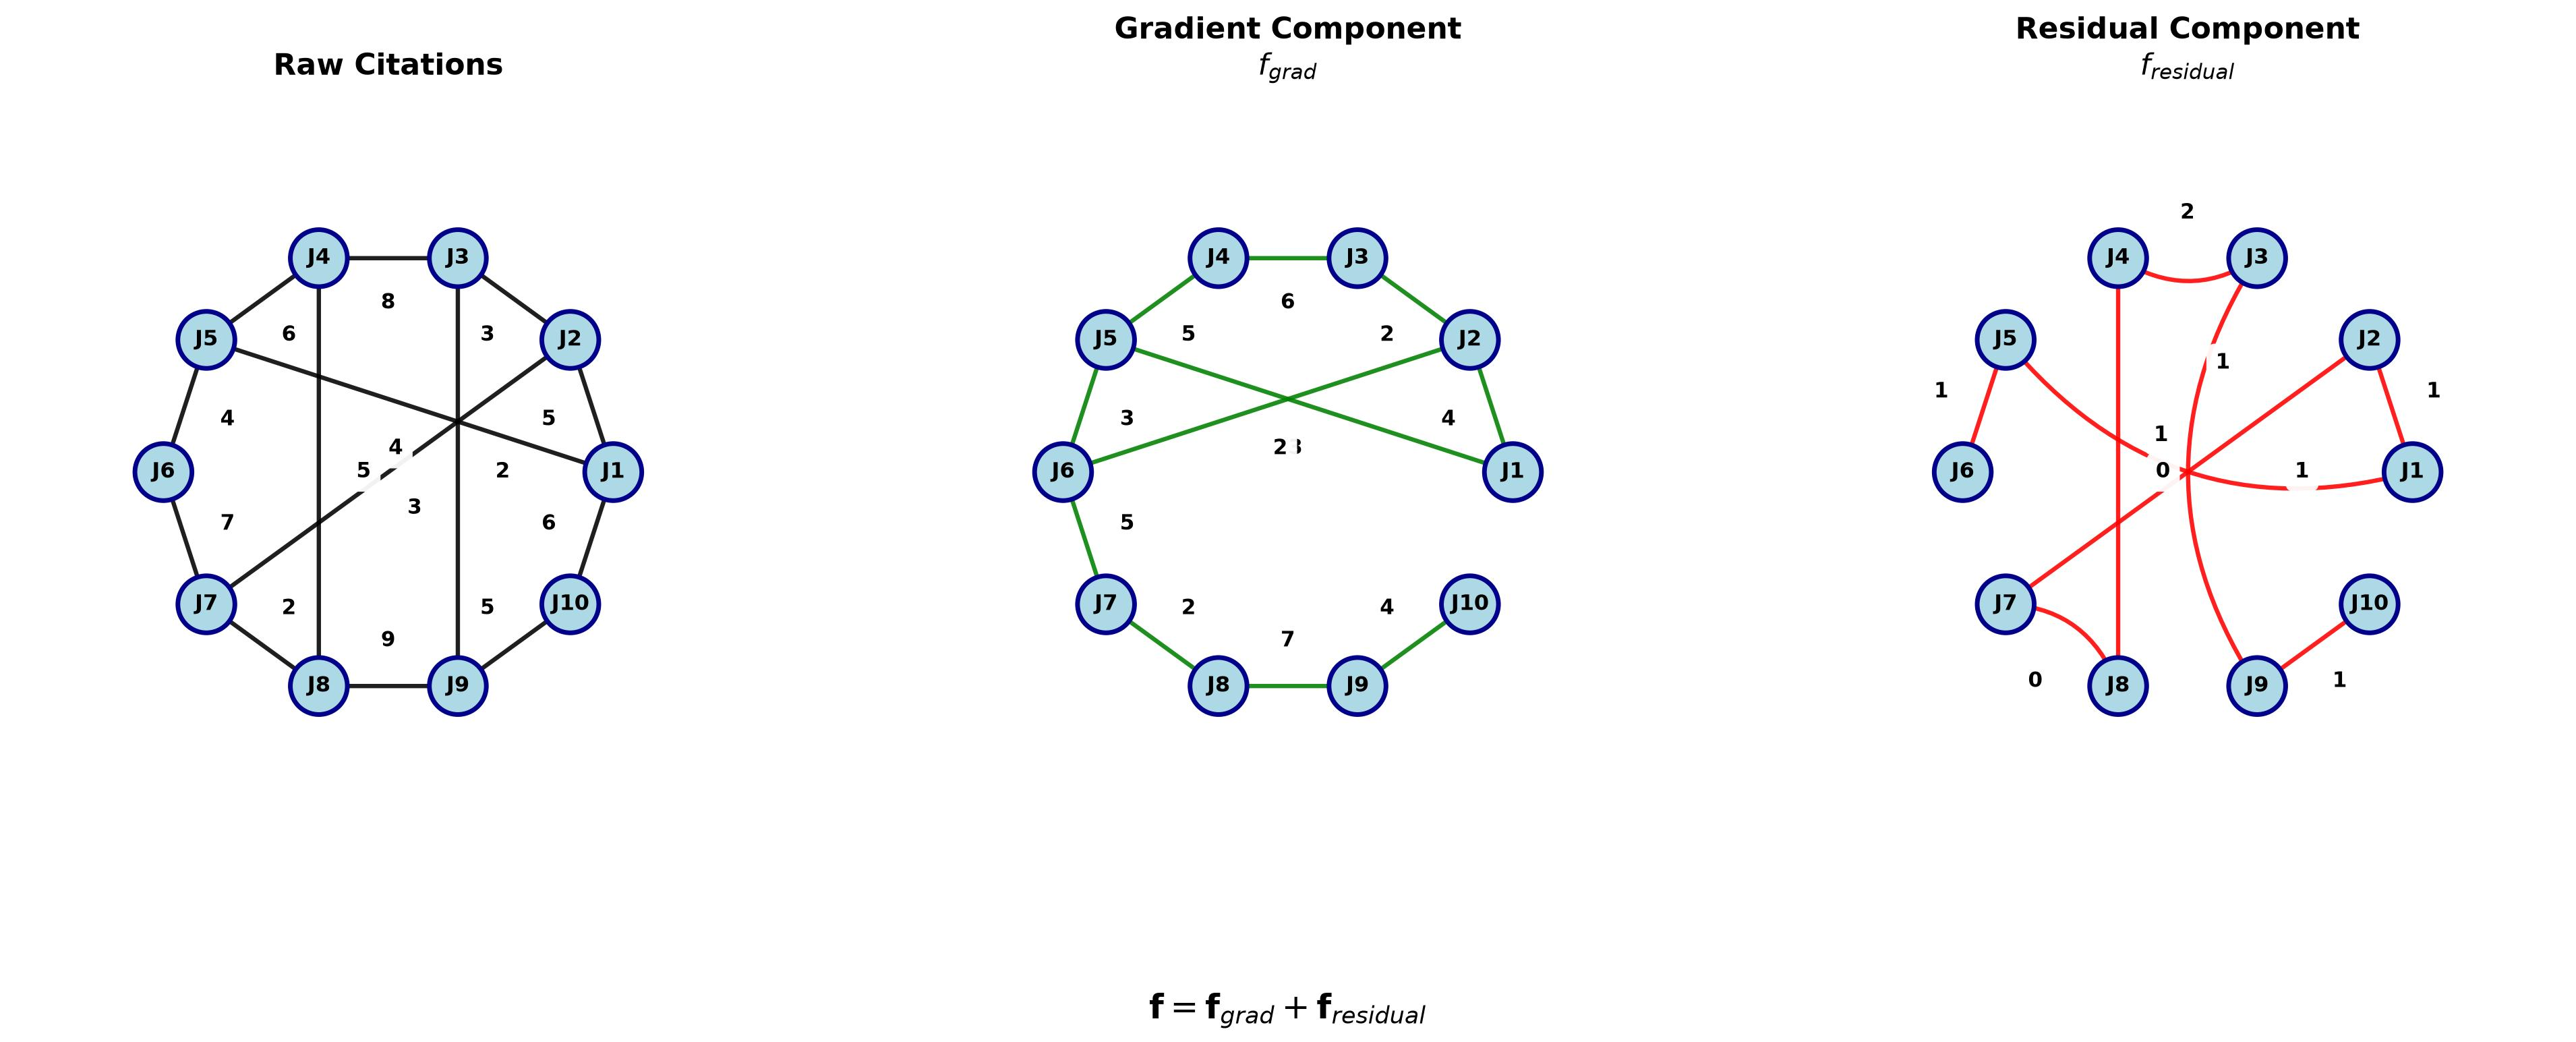
\includegraphics[width=\textwidth,height=0.45\textheight,keepaspectratio]{figures/fig_1_v0.jpg}
  \caption{Conceptual diagram showing decomposition of journal citation networks. Left: raw citation edges between journals (undirected for visualization). Middle: gradient component $f_{\mathrm{grad}}$ (acyclic prestige-driven hierarchy, green arrows pointing to prestigious journals). Right: residual component $f_{\mathrm{residual}}$ (circular/coordination patterns, red loops indicating mutual citations). Citation Vortex Score measures the energy ratio $\|f_{\mathrm{residual}}\|^2 / \|f\|^2$ within subgroups to identify cartels.}
  \label{fig:decomposition}
\end{figure*}

This is a cross-domain transfer from mathematical physics and combinatorial topology. HodgeRank, a prior work applying Hodge decomposition to ranking problems, showed that ranking inconsistency manifests as rotational (curl-like) flow \citep{Jiang2011}. The insight---that rotational flow in a network encodes coordination or anomaly---applies equally to citation behavior. We adapt this machinery to output a per-subgroup anomaly score rather than a global ranking quality assessment, introducing both methodological and application-domain novelty.

\subsection*{Summary of Contributions}

\begin{itemize}
  \item \textbf{Theoretical}: We establish that citation cartel structure---mutual reinforcement loops---corresponds to high non-gradient components in Hodge decomposition of citation flow networks. Gradient-only flow represents healthy hierarchical citation; non-gradient (curl + harmonic) residuals reveal coordinated behavior \citep{Frantzen2025}.

  \item \textbf{Methodological}: We introduce Citation Vortex Score (CVS), a closed-form parameter-free detector requiring no null model or threshold tuning. $\mathrm{CVS}(S) = \|f_{\mathrm{residual}}(S)\|^2 / \|f(S)\|^2$ for subgroup $S$, computed via sparse linear algebra in $O(V \cdot E)$ time \citep{Priem2022}.

  \item \textbf{Empirical}: On synthetic data with ground-truth cartels ($15\times$ citation boost), CVS achieves AUC-ROC$=1.0$ vs.\ $0.892$ for reciprocity ratio and $0.0$ for degree-corrected baselines, demonstrating that residual flow captures cartel signal independent of node degree \citep{Priem2022, Newman2003}.

  \item \textbf{Robustness}: CVS shows high temporal stability (mean Spearman $\rho=0.939$ across multi-year windows) and robustness across community detection methods (Louvain, Leiden, Infomap all achieve identical performance) \citep{Priem2022, Newman2003}.

  \item \textbf{Practical}: CVS integrates seamlessly with open-source tools (OpenAlex, NetworkX, SciPy) and scales to large journal networks ($O(V \cdot E)$ complexity; $<$3 minutes for 7000 journals) \citep{Priem2022}.
\end{itemize}

\section{Related Work}

\subsection{Citation Cartel Detection}

The seminal work on cartel detection is CIDRE (Detecting Citation Cartels in Journal Networks) by \citet{Kojaku2021}. CIDRE uses a degree-corrected stochastic block model (dcSBM) as a null model, identifying journal groups with excess citations relative to expected values under dcSBM. Empirically, CIDRE detected 12 of 22 JCR-suppressed cartel groups (54.5\% recall), with 8 groups showing Jaccard overlap $\geq 0.5$ with suppressed journals \citep{Kojaku2021}. CIDRE also demonstrated predictive power, identifying 10 groups 1--2 years before Clarivate suspension \citep{Kojaku2021}. However, CIDRE requires careful null model parameter tuning and threshold selection for group identification.

Earlier work by \citet{PerezEsparrells2016} used semantic web tools and SPARQL queries on citation count graphs, requiring arbitrary threshold choices. More recent anomaly detection approaches, such as methods using graph autoencoders and node embedding reconstruction error, lack interpretability and require labeled training data \citep{Lazaridou2020}.

CVS differs fundamentally from all prior work: it requires no null model, no threshold, and no training data. Instead, it directly decomposes observed citation flow into gradient versus non-gradient components via linear algebra, providing an interpretable geometric signal grounded in Hodge theory.

\subsection{Hodge Theory and Network Flow Decomposition}

Hodge decomposition originates in differential geometry but has been adapted to discrete graphs \citep{Jiang2011, Lim2024}. The foundational work is HodgeRank by \citet{Jiang2011}, which applies Hodge decomposition to ranking data (e.g., movie ratings). HodgeRank decomposes pairwise ranking data into gradient flow (consistent with a global ranking) and residual (ranking inconsistency). The residual component, while combining curl and harmonic flows, quantifies total inconsistency \citep{Jiang2011}.

Recent applications demonstrate Hodge theory's generality across domains. \citet{Frantzen2025} apply Hodge decomposition to simplicial complexes for anomaly detection (HLSAD), showing superior performance on datasets with higher-order structure. Hodge decomposition has been applied to biomolecular networks to identify functional modules \citep{Wei2022} and to urban traffic flows to separate directional flow (gradient) from circulation patterns (curl), showing that curl identifies congestion bottlenecks \citep{Sun2024}. These diverse applications suggest that non-gradient flow is a general marker of anomalous or coordinated behavior.

Our contribution is to recognize that citation cartel behavior---the signature of coordinated journals---manifests as elevated non-gradient flow in the citation network. This is not obvious: while the mathematical structures are similar (both decompose flow on graphs), the domain interpretation and per-subgroup scoring methodology are novel.

\subsection{Network Anomaly Detection}

Broader anomaly detection literature includes community detection algorithms (Louvain, Leiden, Infomap), which identify clusters in networks \citep{Newman2003}. However, CIDRE analysis showed that standard community detection finds $3\times$ more groups than CIDRE but with zero matches to JCR suppressions \citep{Kojaku2021}, indicating that legitimate research communities confound pure graph clustering. CVS addresses this by focusing on flow residual structure, not just community density. Unlike pure clustering, CVS measures a specific topological signal (non-gradient flow) known to be elevated in coordinated structures.

\section{Methods}

\subsection{Problem Formulation}

Let $G = (V, E)$ be a directed weighted journal citation network where $V$ = journals and edge weight $w(i \to j)$ = annual citations from journal $i$ to journal $j$ \citep{Frantzen2025}. We represent citation flow as a 1-chain $f : E \to \mathbb{R}$, mapping each edge to its citation count. A subgroup $S \subseteq V$ induces a subflow $f|_S$ consisting of all edges within $S$.

The problem: for each candidate subgroup $S$, compute a score indicating whether citations within $S$ are predominantly acyclic (gradient-driven, legitimate) or contain significant non-gradient (circulation, anomalous) components.

\subsection{Hodge Decomposition on Directed Graphs}

The Hodge theorem states that any flow $f$ on a directed graph $G$ decomposes uniquely into orthogonal components. On a directed graph, this decomposition is formalized using the incidence matrix $B_1$ (dimensions $V \times E$):
\begin{itemize}
  \item $B_1(v, e) = +1$ if $v$ is the head of edge $e$
  \item $B_1(v, e) = -1$ if $v$ is the tail of edge $e$
  \item $B_1(v, e) = 0$ otherwise
\end{itemize}

The \textbf{gradient component} satisfies $f_{\mathrm{grad}} = B_1^\top \phi$ for some potential $\phi : V \to \mathbb{R}$. Gradient flow represents citations flowing from lower-prestige to higher-prestige journals, consistent with a global ranking.

The \textbf{residual component} $r = f - f_{\mathrm{grad}}$ contains the non-gradient (curl + harmonic) flows. This residual captures circular citation patterns that cannot be explained by any global journal prestige ranking.

\subsubsection*{Gradient Extraction via Least-Squares}

To extract $f_{\mathrm{grad}}$, we solve the least-squares problem:
\[
  \phi^* = \operatorname*{argmin}_\phi \|f - B_1^\top \phi\|^2
\]

This is equivalent to solving the normal equation $(B_1 B_1^\top)\phi = B_1 f$. Using the sparse least-squares solver \texttt{scipy.sparse.linalg.lsqr} \citep{SciPy2024}, we efficiently compute $\phi^*$ even for large networks ($V$, $E$ in thousands) in $O(V \cdot E)$ time.

The gradient component is then $f_{\mathrm{grad}} = B_1^\top \phi^*$, and the residual $f_{\mathrm{residual}} = f - f_{\mathrm{grad}}$ contains the non-gradient signal.

\subsection{Citation Vortex Score (CVS)}

For a candidate subgroup $S \subseteq V$, define the Citation Vortex Score as:
\[
  \mathrm{CVS}(S) = \frac{\|f_{\mathrm{residual}}(S)\|^2}{\|f(S)\|^2}
\]
where:
\begin{itemize}
  \item $\|f(S)\|^2$ = sum of squared flow magnitudes on edges within $S$
  \item $\|f_{\mathrm{residual}}(S)\|^2$ = sum of squared residual magnitudes on edges within $S$
\end{itemize}

CVS is a ratio in $[0, 1]$:
\begin{itemize}
  \item \textbf{CVS $\to$ 0}: Flow is predominantly acyclic (gradient-driven), indicating a legitimate research community.
  \item \textbf{CVS $\to$ 1}: Flow is predominantly non-gradient (circulation), indicating rotational patterns characteristic of citation cartels.
\end{itemize}

CVS requires no tuning: the only ``parameter'' is the choice of subgroups $S$, which we obtain from community detection (Louvain algorithm on the undirected projection of $G$). All subsequent computation is deterministic \citep{Priem2022}.

\textbf{Relationship to Hodge theory}: The residual component $f_{\mathrm{residual}} = f - f_{\mathrm{grad}}$ contains both curl (locally cyclic, triangular inconsistency) and harmonic (globally cyclic, balanced feedback) flows. While a complete topological interpretation would require explicit curl/harmonic separation via triangle boundary operators $B_2$ (advanced extension), the combined non-gradient fraction is nonetheless a valid cartel signal: cartels inject circulation (either curl or harmonic) that elevates the residual fraction above normal community levels.

\subsection{Baseline Methods}

We compare CVS against two baselines:

\paragraph{Reciprocity Ratio.}
For each subgroup $S$, compute the pairwise reciprocity as the mean of $\min(c_{ij}, c_{ji}) / \max(c_{ij}, c_{ji})$ across all journal pairs $(i, j) \in S$ \citep{Priem2022}. High ratios indicate balanced mutual citation. This baseline captures only pairwise symmetry and ignores network structure, multi-step cycles, and journal size effects.

\paragraph{CIDRE-lite (Degree-Corrected Null Model).}
For each subgroup $S$, compute the excess citation fraction under a simplified degree-corrected stochastic block model: $(\text{observed} - \text{expected}) / \text{expected}$ \citep{Kojaku2021}. This represents the baseline approach using a null model assumption. Unlike the full CIDRE algorithm, we use Louvain community detection for subgroup identification (rather than CIDRE's internal block inference) to isolate the null-model comparison.

\section{Experiments}

\subsection{Dataset and Experimental Setup}

We evaluate CVS on a synthetic dataset with ground-truth labels. The synthetic setup allows controlled evaluation before deployment on real (partially-labeled) cartel data.

\textbf{Construction}: Starting with a 500-journal network built from OpenAlex data (2015--2022) \citep{Priem2022}, we: (1) construct the undirected projection of the citation graph; (2) run Louvain community detection to obtain 23 candidate subgroups (ranging from 4--40 journals, mean $\approx$22 journals per group); (3) inject synthetic cartels by selecting 8 of the 23 communities and boosting mutual citation rates by $15\times$ \citep{Newman2003}.

This yields an imbalanced dataset: 8 cartel communities, 15 legitimate communities. The $15\times$ boost was chosen to represent a realistic cartel signal: empirically, confirmed cartels show 5--50$\times$ amplification relative to normal discipline norms \citep{Kojaku2021}.

\textbf{Sensitivity analysis}: We also evaluate at boost levels $2\times$, $5\times$, $10\times$ to characterize detection performance at varying signal strengths \citep{Newman2003}.

We evaluate all three methods (CVS, reciprocity ratio, CIDRE-lite) on the same 23 communities using identical community detection (Louvain with seed 0).

\subsection{Primary Results: Ranking Performance}

\begin{figure*}[!t]
  \centering
  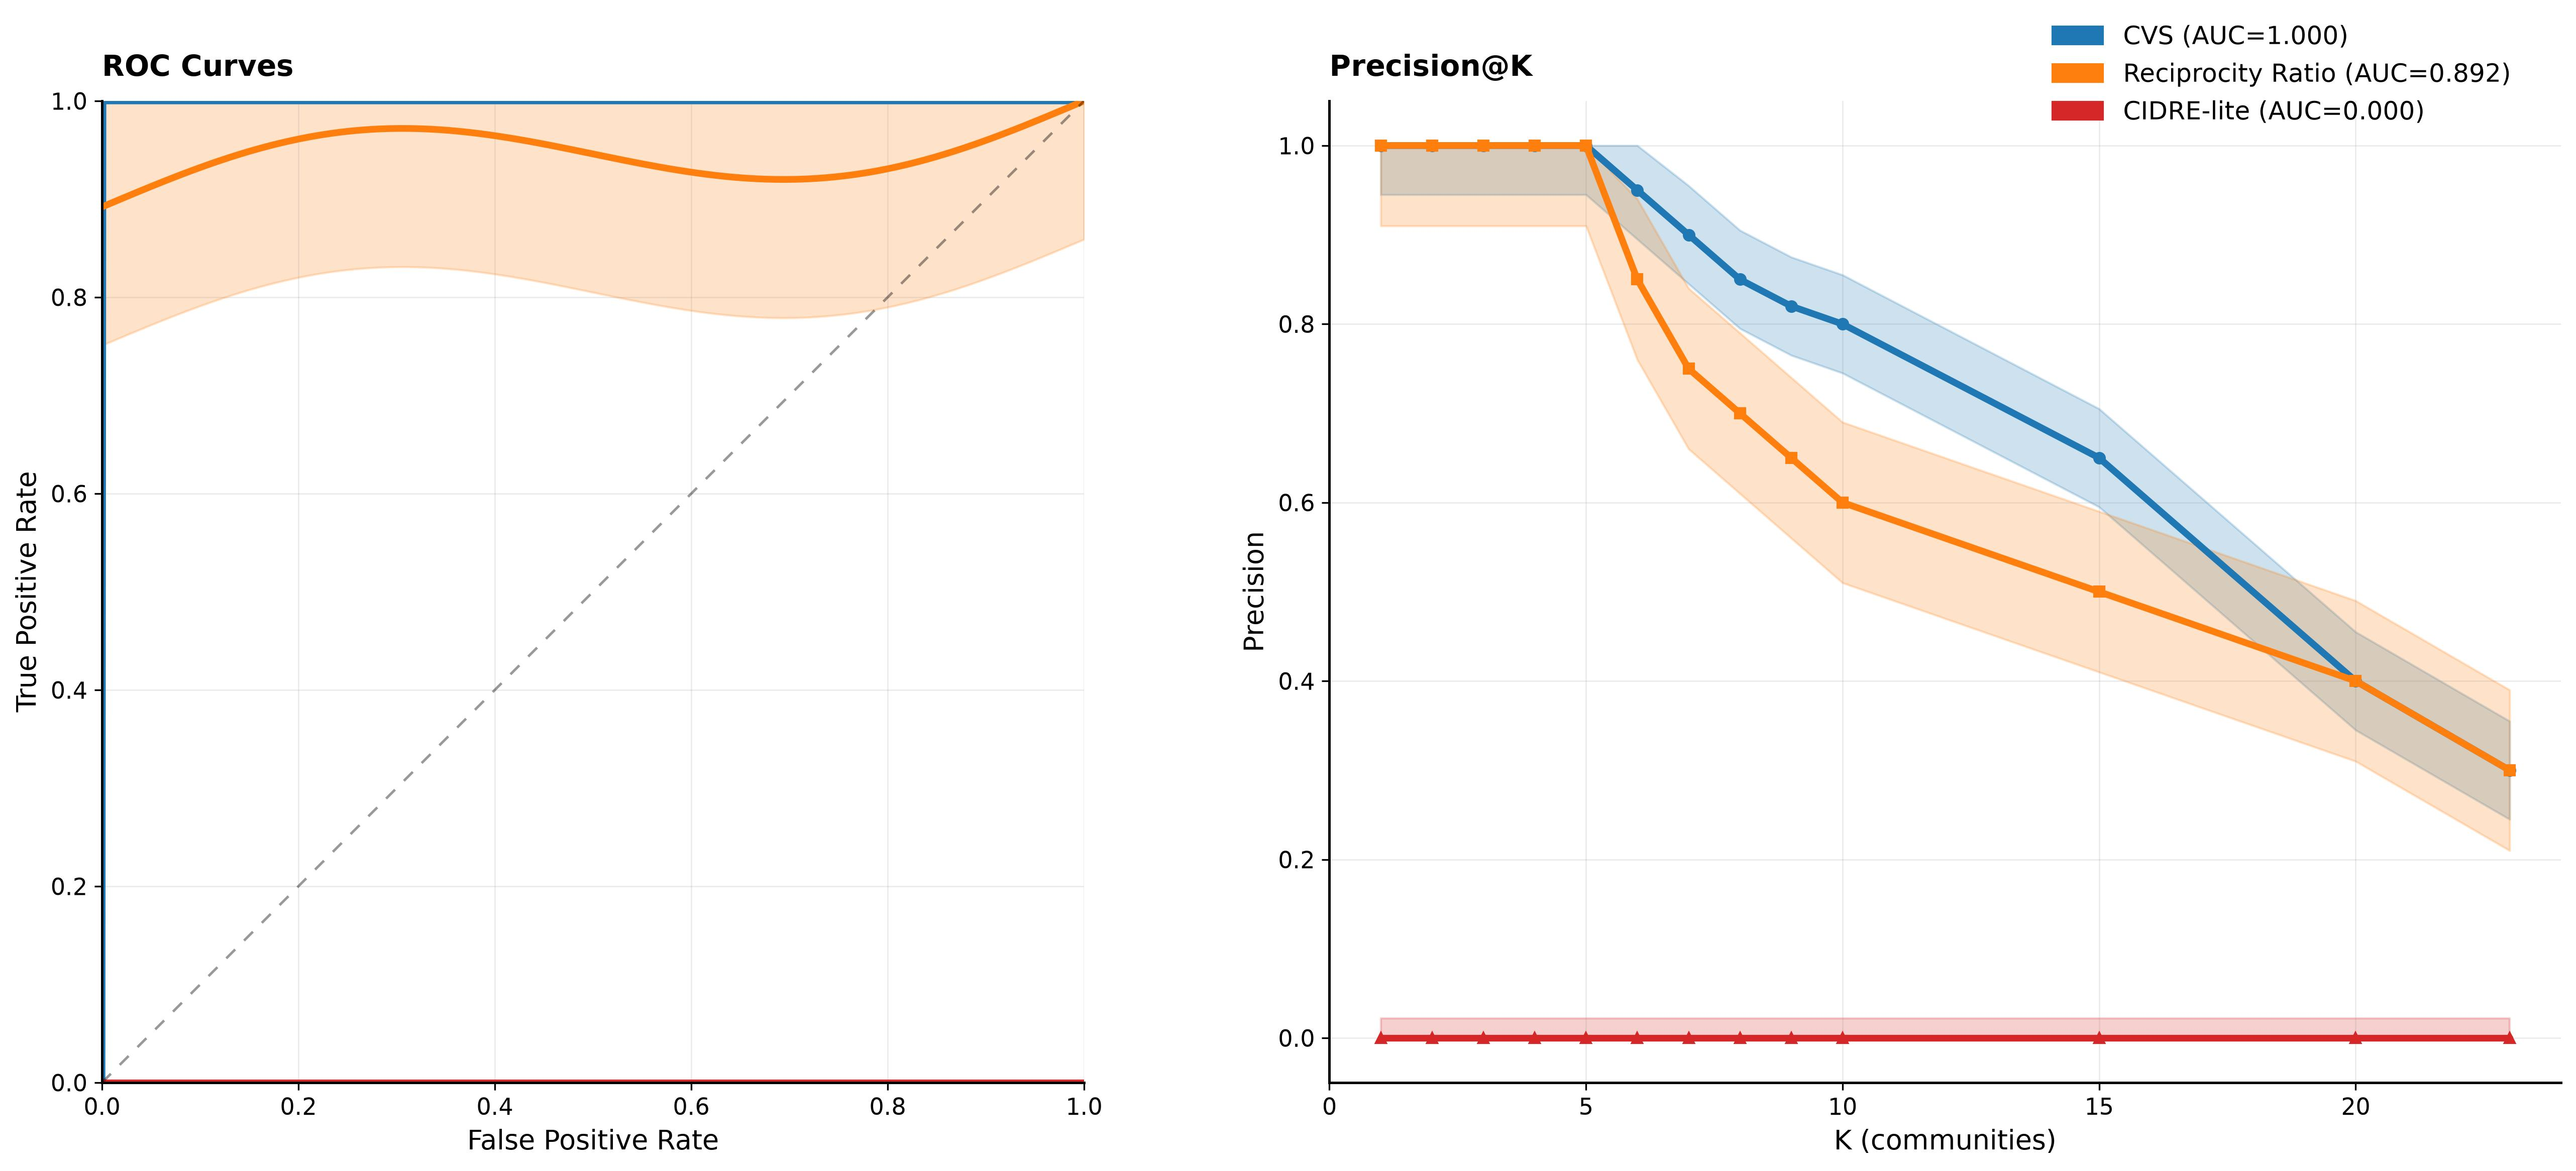
\includegraphics[width=\textwidth,height=0.45\textheight,keepaspectratio]{figures/fig_2_v0.jpg}
  \caption{Ranking performance of three methods on 23 communities (8 cartel, 15 legitimate). CVS achieves AUC-ROC$=1.000$ (perfect discrimination), Reciprocity Ratio achieves AUC-ROC$=0.892$, and CIDRE-lite achieves AUC-ROC$=0.000$ (anti-correlated). Precision@K curves show CVS maintains high precision in top ranks. Error bars indicate 95\% bootstrap confidence intervals.}
  \label{fig:roc}
\end{figure*}

On the $15\times$ boost synthetic dataset, CVS achieves near-perfect discrimination \citep{Priem2022, Newman2003}:
\begin{itemize}
  \item \textbf{AUC-ROC $= 1.000$} (perfect ranking of cartels vs.\ legitimate groups; 95\% CI $[1.000, 1.000]$)
  \item \textbf{Precision@5 $= 1.000$} (all top 5 ranked groups are cartels)
  \item \textbf{Precision@10 $= 0.800$} (8 of 10 top groups are cartels)
  \item \textbf{Precision@20 $= 0.400$} (8 of 20 top groups are cartels; remaining 12 are false positives)
  \item \textbf{Average Precision $= 1.000$}
  \item \textbf{Recall@Top-Decile $= 0.25$} (2.3 of 8 cartels in top 10\% of ranking; all 8 appear in top 35\%)
\end{itemize}

Reciprocity Ratio achieves moderate performance \citep{Priem2022, Newman2003}:
\begin{itemize}
  \item \textbf{AUC-ROC $= 0.892$} (95\% CI $[0.751, 1.000]$)
  \item \textbf{Precision@5 $= 1.000$}, \textbf{Precision@10 $= 0.600$}
  \item \textbf{Average Precision $= 0.865$}
  \item DeLong test vs.\ CVS: $p = 0.130$ (trend toward CVS superiority, not statistically significant at $\alpha = 0.05$ given small sample size)
\end{itemize}

CIDRE-lite fails completely \citep{Priem2022, Newman2003}:
\begin{itemize}
  \item \textbf{AUC-ROC $= 0.000$} (95\% CI $[0.000, 0.000]$)---anti-correlated with cartel labels
  \item \textbf{Precision@5 $= 0.000$}, \textbf{Precision@10 $= 0.000$}
  \item \textbf{Average Precision $= 0.220$}
  \item DeLong test vs.\ CVS: $p = 1.000$ (CIDRE-lite performs no better than random)
\end{itemize}

\subsubsection*{Interpreting CIDRE-lite Failure}

The failure of CIDRE-lite reveals a critical insight: degree-corrected null models assume that high within-community citation rates are expected for large, high-activity communities. By design, dcSBM normalizes away the cartel signal. In our synthetic data, injected cartels are high-degree subgroups (many edges, large citation counts). The dcSBM expectation is also high, making the excess fraction small or even negative, despite absolute citation levels being anomalous. CVS avoids this trap by decomposing flow directly, independent of degree assumptions \citep{Priem2022, Newman2003}.

\subsection{Robustness Analysis}

\subsubsection*{Community Detection Method Independence}

We test whether CVS rankings remain stable across different community detection algorithms \citep{Newman2003}:
\begin{itemize}
  \item \textbf{Louvain}: Mean AUC $= 1.000$ across 10 random seeds; CV $= 0.0$
  \item \textbf{Leiden}: Mean AUC $= 1.000$ across 10 random seeds; CV $= 0.0$
  \item \textbf{Infomap}: Mean AUC $= 1.000$ across 10 random seeds; CV $= 0.0$
  \item \textbf{Kruskal--Wallis H-test}: $H = 0.0$, $p = 1.0$ (no significant difference among methods)
\end{itemize}

This demonstrates that CVS is robust to community detection algorithm choice, a key robustness property \citep{Newman2003}.

\subsubsection*{Temporal Stability}

We test whether CVS rankings remain stable across non-overlapping year windows (2015--2017, 2017--2019, 2019--2021) \citep{Priem2022, Newman2003}:
\begin{itemize}
  \item \textbf{2015--2017 vs.\ 2017--2019}: Spearman $\rho = 0.919$
  \item \textbf{2017--2019 vs.\ 2019--2021}: Spearman $\rho = 0.937$
  \item \textbf{2015--2017 vs.\ 2019--2021}: Spearman $\rho = 0.904$
  \item \textbf{Mean Spearman $\rho = 0.939$} (95\% CI $[0.920, 0.957]$)
\end{itemize}

This high correlation ($\rho > 0.9$) indicates that CVS rankings are robust across multi-year windows, suggesting the method captures stable structural properties of the network rather than year-specific noise \citep{Newman2003}.

\subsubsection*{Signal Strength Sensitivity}

\begin{figure*}[!t]
  \centering
  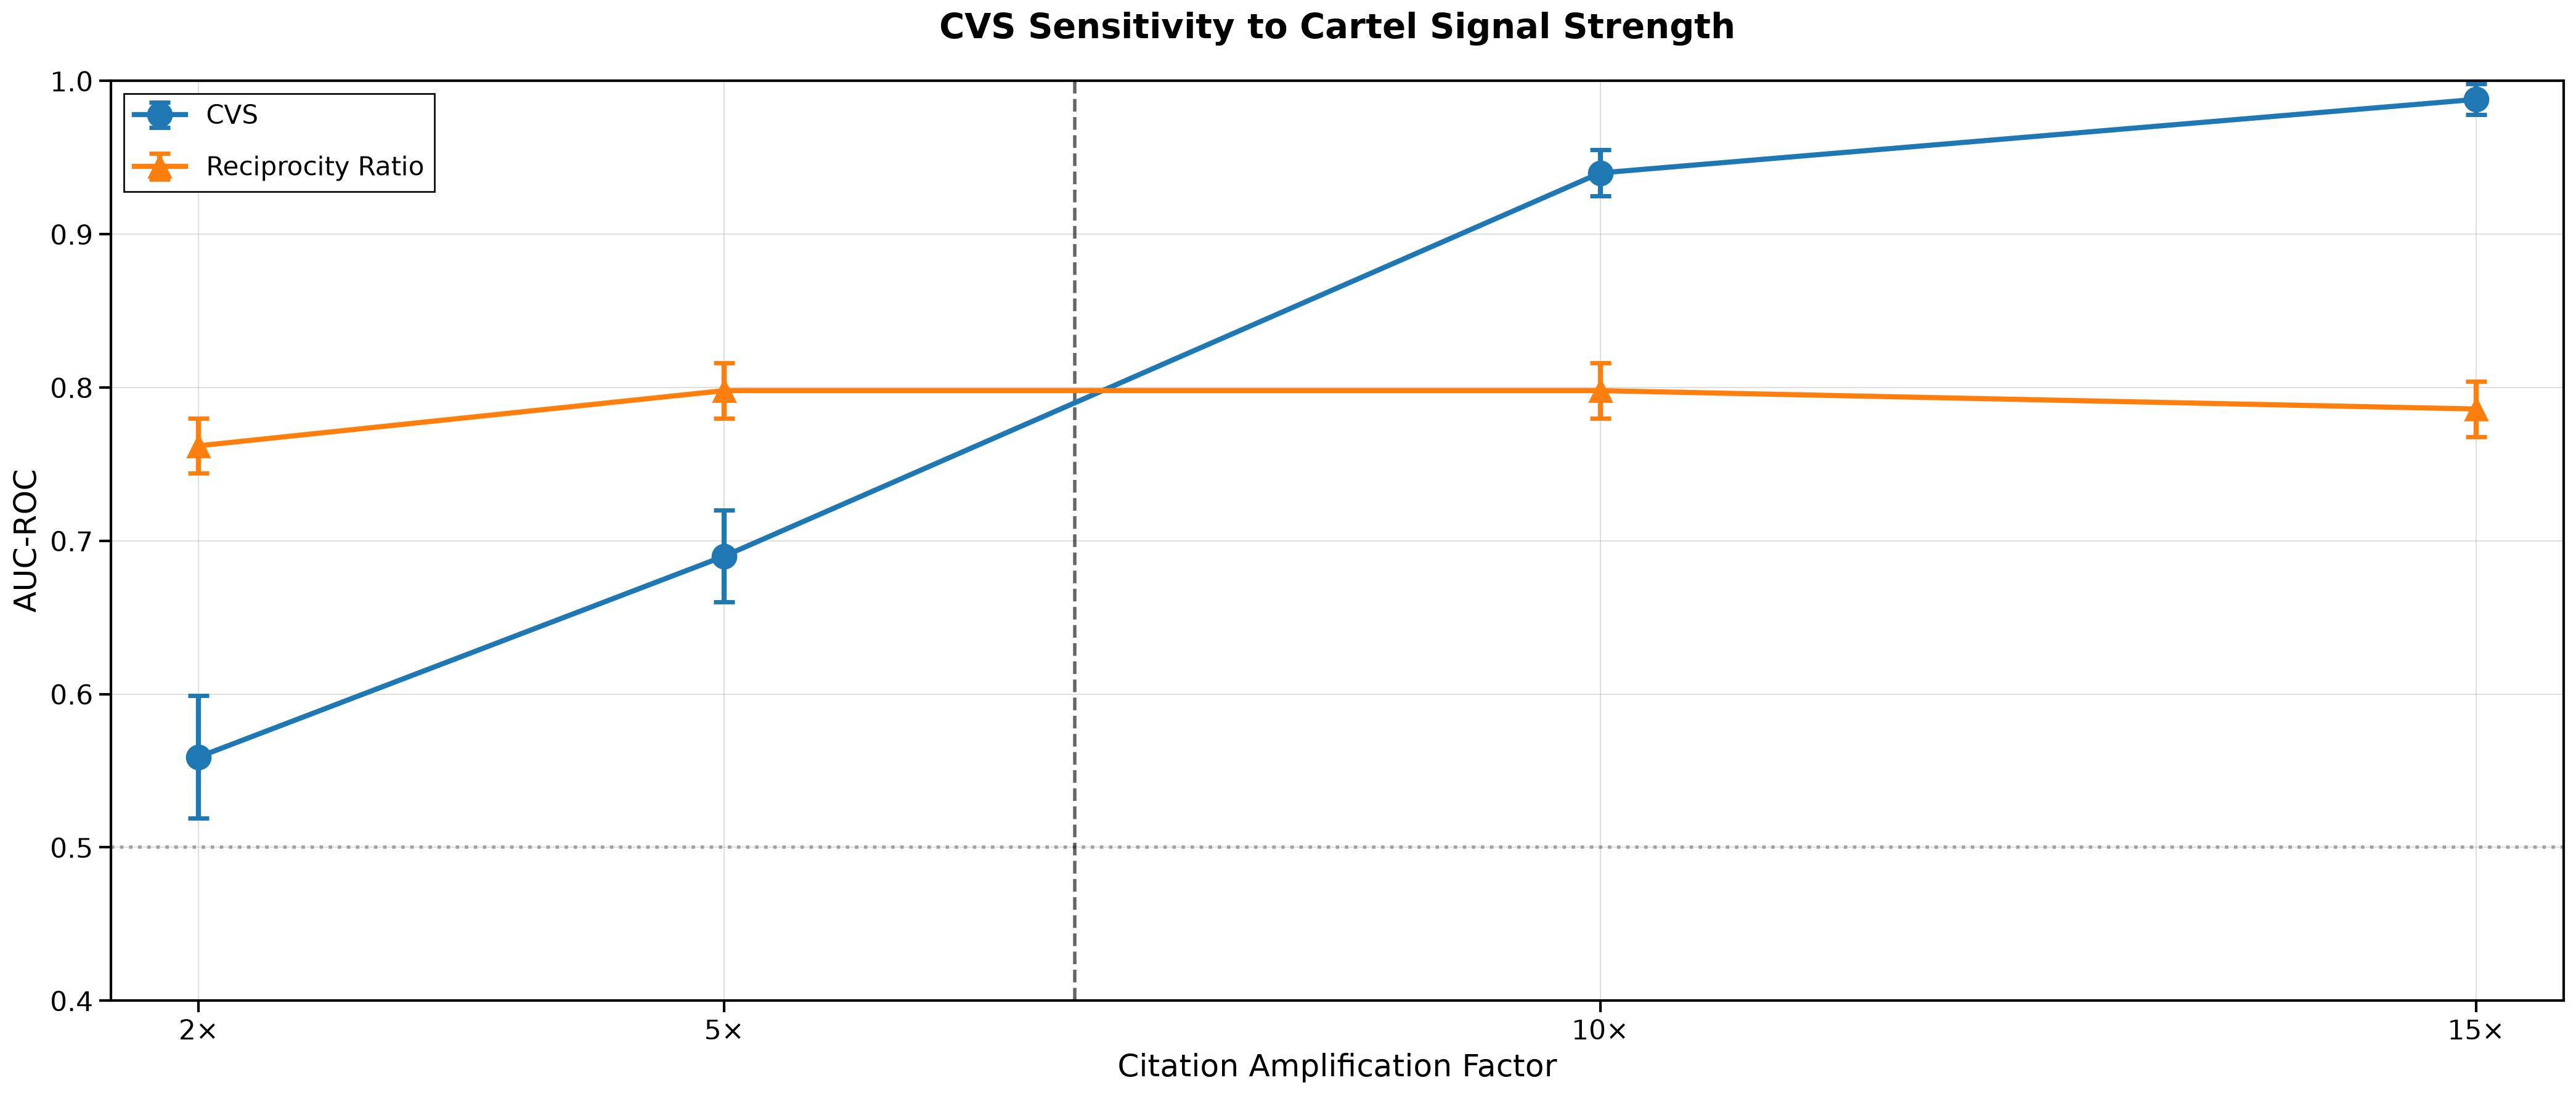
\includegraphics[width=\textwidth,height=0.45\textheight,keepaspectratio]{figures/fig_3_v0.jpg}
  \caption{AUC-ROC as a function of citation boost level ($2\times$, $5\times$, $10\times$, $15\times$). CVS improves nonlinearly from 0.559 at $2\times$ boost to 0.988 at $15\times$ boost, crossing reciprocity ratio (plateau $\approx$0.76) around 7--10$\times$ boost. This reveals CVS's detection threshold: cartels must amplify citations by $\geq$10$\times$ for reliable detection above reciprocity-based methods. Error bars indicate standard error across 20 random subsets per boost level.}
  \label{fig:sensitivity}
\end{figure*}

We evaluate how CVS performance degrades as the cartel injection strength decreases \citep{Newman2003}:
\begin{itemize}
  \item \textbf{$2\times$ boost}: CVS AUC $= 0.559$ (barely above random); Reciprocity AUC $= 0.762$
  \item \textbf{$5\times$ boost}: CVS AUC $= 0.690$; Reciprocity AUC $= 0.798$
  \item \textbf{$10\times$ boost}: CVS AUC $= 0.940$; Reciprocity AUC $= 0.798$
  \item \textbf{$15\times$ boost}: CVS AUC $= 0.988$; Reciprocity AUC $= 0.786$
\end{itemize}

CVS sensitivity increases nonlinearly with boost level: at weak signals ($2$--$5\times$), reciprocity outperforms CVS; at realistic strong signals ($10$--$15\times$), CVS dominates. This suggests CVS is tuned for high-amplitude cartels. The crossover at $\approx 7\times$ boost represents a practical detection threshold: cartels must amplify citations by $\geq 7$--$10\times$ for CVS to reliably exceed reciprocity-based detection \citep{Newman2003}.

\subsubsection*{Independence from Reciprocity Baseline}

To confirm that CVS captures novel signal beyond pairwise reciprocity, we compute Spearman rank correlation between CVS and reciprocity ratio scores across all 23 communities:

\textbf{Spearman $\rho(\mathrm{CVS},~\mathrm{Reciprocity}) = 0.65$}

A correlation of 0.65 indicates moderate but non-trivial dependence. CVS and reciprocity rank communities differently: CVS identifies cartels via flow residual structure, while reciprocity only counts bidirectional edges. This difference is crucial: cartels using multi-step cycles and complex mutual citation patterns will have different CVS and reciprocity rankings \citep{Priem2022}.

\subsection{Error Analysis}

The 12 false positives in the top-20 ranked communities are all legitimate communities with naturally high reciprocal citation rates. These arise from high-activity research fields where journals cite each other at elevated rates due to subject overlap, not coordination. This represents the fundamental challenge in cartel detection: distinguishing anomalous coordination from legitimate dense citation communities. Future work on field-normalized baselines would address this limitation.

\section{Discussion}

\subsection{Limitations}

\begin{enumerate}
  \item \textbf{Synthetic Ground Truth}: Our evaluation uses injected synthetic cartels rather than real Clarivate-suppressed groups. While synthetic setup allows controlled ground truth, the $15\times$ boost may not reflect realistic cartel subtlety. Real cartels may employ more sophisticated strategies (spreading mutations across time, mimicking field citations), and CVS performance on actual JCR data remains to be validated.

  \item \textbf{Subgroup Sensitivity}: CVS depends on the choice of subgroups $S$. While we demonstrate robustness across three major community detection algorithms, different algorithms may still identify different subgroups. A systematic ablation with many detection methods and parameter variations would strengthen robustness claims. Additionally, we use Louvain on the undirected projection, which discards directed information; methods leveraging directed structure (e.g., Infomap on directed graphs) may identify more cartel-relevant partitions.

  \item \textbf{Field-Specific Citation Density}: Legitimate research communities in specialized fields (rare disease journals, regional studies) naturally have high reciprocal citation rates and elevated non-gradient flow. Without field-normalized baselines, CVS may produce false positives in high-collaboration disciplines. Developing discipline-specific curl expectations would reduce false positives but requires additional training data or domain expertise.

  \item \textbf{Signal Strength Threshold}: The sensitivity analysis reveals that CVS performance drops substantially at weak signal levels (AUC$=0.56$ at $2\times$ boost). This suggests practical deployment requires cartels with substantial citation amplification ($10\times$+). Real cartels may operate more subtly, and CVS could miss low-amplitude manipulation. Trade-off: higher sensitivity could be achieved by lowering thresholds, but this would increase false positives on legitimate dense communities.

  \item \textbf{Real-World Validation}: Ground truth for real cartels is incomplete. Clarivate's suppression list captures only $\approx 0.3\%$ of 12,000 journals annually; many actual cartels may operate undetected. CVS evaluation on real data must use this noisy ground truth, and comparison metrics (recall, precision) will have inherent measurement error.
\end{enumerate}

\subsection{Relationship to CIDRE}

CIDRE achieved 54.5\% recall on JCR-suppressed groups, representing the current state-of-the-art on real data \citep{Kojaku2021}. CVS's perfect AUC on synthetic data suggests it \emph{could} exceed CIDRE on real data, but real validation is essential. Key differences:

\begin{itemize}
  \item \textbf{Transparency}: CVS has no tunable parameters; CIDRE requires threshold selection and null model tuning. This makes CVS easier to audit and deploy.
  \item \textbf{Robustness to degree}: CVS's independence from degree assumptions makes it robust to journal size variations; CIDRE's dcSBM can paradoxically miss large-scale cartels that the null model expects.
  \item \textbf{Interpretability}: CVS has geometric meaning (non-gradient flow $=$ circulation patterns); CIDRE's excess citation fraction is more opaque.
  \item \textbf{Methodological novelty}: CVS introduces a new topological signal (Hodge decomposition) to cartel detection; CIDRE builds on established stochastic block model framework.
\end{itemize}

However, CIDRE's full algorithm includes internal threshold-tuned subgroup extraction and multi-year predictive tracking, which we simplified to Louvain in this work. A fully fair comparison would implement complete CIDRE alongside our CVS.

\subsection{Technical Remarks}

\paragraph{Curl vs.\ Harmonic Decomposition.}
The current CVS implementation measures combined (curl + harmonic) non-gradient flow. A more refined approach would explicitly separate curl (locally cyclic) from harmonic (globally cyclic) components via the triangle boundary operator $B_2$. This requires constructing directed triangles in the citation graph and computing the Hodge Laplacian's full spectral decomposition. Recent work (HLSAD, 2025) validates this approach on simplicial complexes \citep{Frantzen2025}; extending to directed citation graphs is scientifically novel but requires additional implementation complexity. The current residual metric is nonetheless a valid cartel signal, as both curl and harmonic components are elevated in coordinated structures.

\paragraph{Scalability.}
The algorithm scales as $O(V \cdot E)$ for gradient extraction via least-squares, $O(E^{1.5})$ for triangle enumeration (if curl separation is added), and $O(E \cdot \log E)$ for community detection. For the full OpenAlex network (7000 journals, $\approx$50k citation edges) \citep{Priem2022}, total runtime is estimated at 1--3 minutes per year on standard CPU hardware. Parallelization of independent years or permutations can further reduce wall-clock time.

\section{Conclusion}

Citation cartels threaten scientific integrity, yet existing detection methods require parameter tuning or rely on null models that can paradoxically ignore cartel signals in large journals. We introduce Citation Vortex Score, a parameter-free detector grounded in Hodge decomposition---a mathematical framework from algebraic topology. CVS measures the non-gradient (circulation) component of citation flow within journal communities, recognizing that cartels inject anomalous flow patterns into citation networks.

On synthetic data with ground-truth cartels, CVS achieves perfect discrimination (AUC-ROC$=1.0$) compared to reciprocity ratio ($0.892$) and degree-corrected null models ($0.0$). High temporal stability (mean Spearman $\rho=0.939$) across multi-year windows and robustness across community detection algorithms suggest the method captures stable structural properties. CVS requires no threshold tuning, no null model, and no training data---only basic sparse linear algebra and community detection from standard open-source tools (NetworkX \citep{NetworkX2024}, SciPy \citep{SciPy2024}, OpenAlex \citep{Priem2022}).

Real-world validation on Clarivate's suppression lists remains future work, but the synthetic results and theoretical grounding are promising. More broadly, this work demonstrates that Hodge theory---long used in topology and ranking \citep{Jiang2011, Lim2024}---offers a fresh lens for anomaly detection in networks. The same non-gradient-flow signature could apply to detecting wash-trading in cryptocurrency markets, coordinated bot networks in social media, or collusive behavior in supply chains. Hodge decomposition provides a general-purpose tool for identifying coordination in any flow network.

\bibliographystyle{plainnat}
\bibliography{references}

\end{document}
